% Five-stage training curriculum (Chapter 6, sec:sns_curriculum).
% Compile: pdflatex -output-directory=.. sns_curriculum.tex
\documentclass[border=6pt]{standalone}
\usepackage[T1]{fontenc}
\usepackage{mathpazo}
\usepackage{tikz}
\usetikzlibrary{arrows.meta, positioning}
\begin{document}
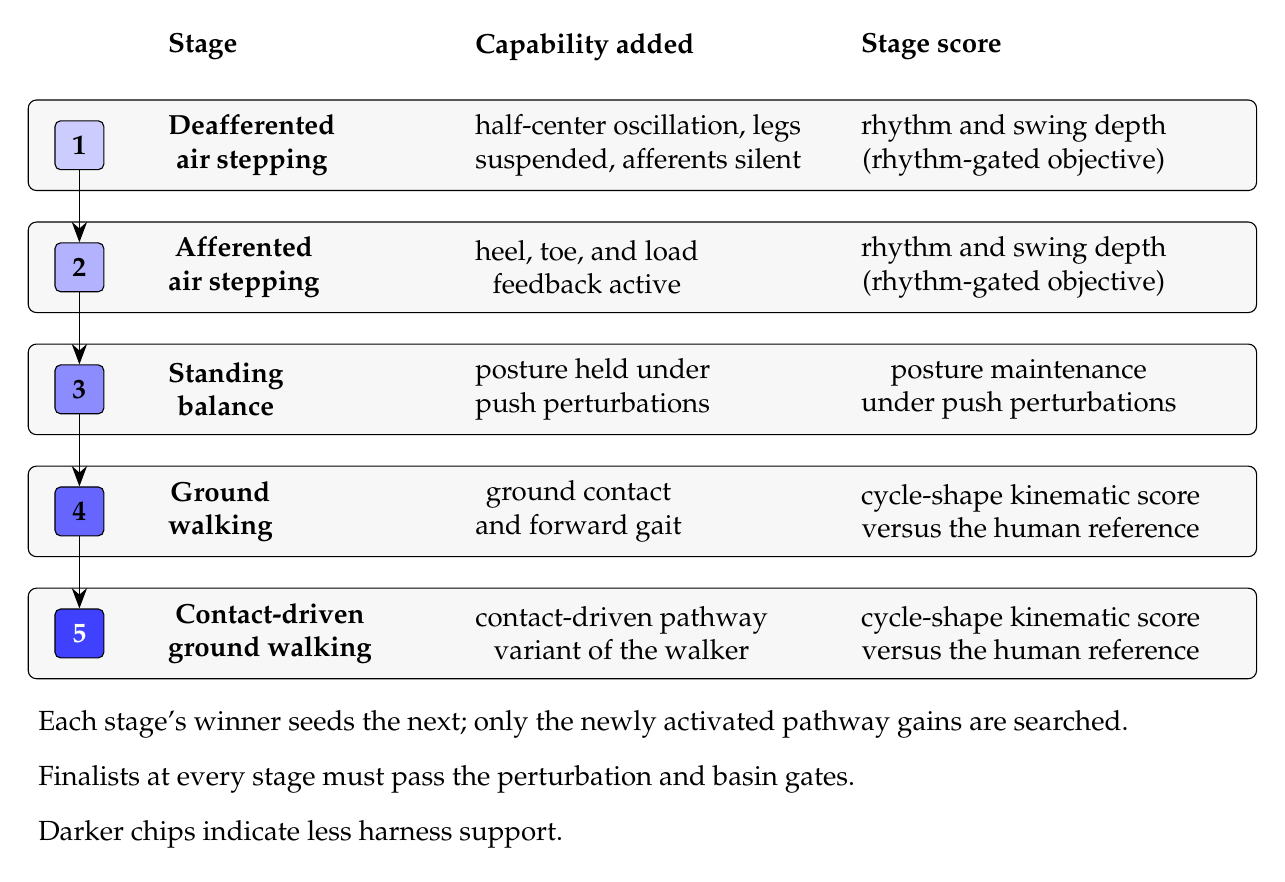
\begin{tikzpicture}[
  font=\normalsize,
  row/.style={draw, rounded corners=3pt, fill=black!3, inner sep=0pt,
              minimum width=15.6cm, minimum height=1.15cm},
  chip/.style={draw, rounded corners=2pt, minimum width=0.62cm,
               minimum height=0.62cm, font=\normalsize\bfseries},
  arrow/.style={-{Stealth[length=2.6mm]}, thin},
  lab/.style={align=center, inner sep=2pt},
  head/.style={font=\normalsize\bfseries, inner sep=2pt},
]

% Column headers
\node[head, anchor=west] at (2.0,2.35) {Stage};
\node[head, anchor=west] at (5.9,2.35) {Capability added};
\node[head, anchor=west] at (10.8,2.35) {Stage score};

% Stage rows
\node[row] (s5) at (8.1,-5.1) {};
\node[row] (s4) at (8.1,-3.55) {};
\node[row] (s3) at (8.1,-2.0) {};
\node[row] (s2) at (8.1,-0.45) {};
\node[row] (s1) at (8.1,1.1) {};

\node[chip, fill=blue!20] (c1) at (0.95,1.1) {1};
\node[chip, fill=blue!30] (c2) at (0.95,-0.45) {2};
\node[chip, fill=blue!45] (c3) at (0.95,-2.0) {3};
\node[chip, fill=blue!60]  (c4) at (0.95,-3.55) {4};
\node[chip, fill=blue!75, text=white] (c5) at (0.95,-5.1) {5};

\node[lab, anchor=west, font=\normalsize\bfseries] at (2.0,1.1) {Deafferented\\air stepping};
\node[lab, anchor=west] at (5.9,1.1) {half-center oscillation, legs\\suspended, afferents silent};
\node[lab, anchor=west] at (10.8,1.1) {rhythm and swing depth\\(rhythm-gated objective)};

\node[lab, anchor=west, font=\normalsize\bfseries] at (2.0,-0.45) {Afferented\\air stepping};
\node[lab, anchor=west] at (5.9,-0.45) {heel, toe, and load\\feedback active};
\node[lab, anchor=west] at (10.8,-0.45) {rhythm and swing depth\\(rhythm-gated objective)};

\node[lab, anchor=west, font=\normalsize\bfseries] at (2.0,-2.0) {Standing\\balance};
\node[lab, anchor=west] at (5.9,-2.0) {posture held under\\push perturbations};
\node[lab, anchor=west] at (10.8,-2.0) {posture maintenance\\under push perturbations};

\node[lab, anchor=west, font=\normalsize\bfseries] at (2.0,-3.55) {Ground\\walking};
\node[lab, anchor=west] at (5.9,-3.55) {ground contact\\and forward gait};
\node[lab, anchor=west] at (10.8,-3.55) {cycle-shape kinematic score\\versus the human reference};

\node[lab, anchor=west, font=\normalsize\bfseries] at (2.0,-5.1) {Contact-driven\\ground walking};
\node[lab, anchor=west] at (5.9,-5.1) {contact-driven pathway\\variant of the walker};
\node[lab, anchor=west] at (10.8,-5.1) {cycle-shape kinematic score\\versus the human reference};

\foreach \i/\j in {c1/c2, c2/c3, c3/c4, c4/c5} {
  \draw[arrow] (\i) -- (\j);
}

\node[lab, anchor=west] at (0.35,-6.25)
  {Each stage's winner seeds the next; only the newly activated pathway gains are searched.};
\node[lab, anchor=west] at (0.35,-6.95)
  {Finalists at every stage must pass the perturbation and basin gates.};
\node[lab, anchor=west] at (0.35,-7.65)
  {Darker chips indicate less harness support.};

\end{tikzpicture}
\end{document}
